%\renewcommand{\Titulo}{Intelligent weighing system ~}

\begin{frame}{\citetitle{MarcoNuno_CongArbEsp_2019_09_01} \footnotemark (1)}
\begin{block}{Problem description} 


%\begin{columns}
%\begin{column}{0.5\textwidth}

	\begin{itemize}
	\item Nowadays, the integration of sensors for monitoring, diagnosis, and treatment in people with a disease facilitated the development of very varied platforms and applications. 
\note[item]{\scriptsize This integration allows health professionals to achieve significant advances in a faster and more effective way.}
    \item Technological tools would aid health institutions in acquiring viable and reliable data for the treatment of obesity. 
%\note[item]{\scriptsize ... would help to prevent chronic diseases for those who already suffer from any of them.}
    \item We propose an intelligent low-cost weight system based on Raspberry Pi microcomputer. 
\note[item]{\scriptsize The device obtains the parameters required to calculate the basal metabolic rate of people and combined with the type of physical activity performed, a recommended meal plan is generated. }
\item This recommendation would aid the user in maintaining good health by helping to control diseases such as obesity, diabetes, and high blood pressure.
	\end{itemize}
\end{block} 
\footnotetext[1]{\fullcite{MarcoNuno_CongArbEsp_2019_09_01}}
\setcounter{footnote}{0}
\end{frame}

\begin{frame}{\citetitle{MarcoNuno_CongArbEsp_2019_09_01} (2)}


% 
%The system uses the sensors to acquire the user's body parameters. The GUI represents the actions to be performed by the user and the results produced by the device without having physical contact with it. The Python Eel library allows access to Python's capabilities via HTML and JavaScript, which makes it perfect for developing GUIs using the full potential of HTML, HTML5, and JavaScript.  The system requires a remote connection to a database server for the design and functionality of the device. This interface only shows the logo of the device and a welcome message that invites you to initiate the interaction through the voice command "HELLO". The device will ask the user the age, which with the voice, will respond only by saying the user's age (one single number). 

\note[item]{\scriptsize The system uses the sensors to acquire the user's body parameters. The GUI represents the actions to be performed by the user and the results produced by the device without having physical contact with it.}

\note[item]{\scriptsize The system requires a remote connection to a database server for the design and functionality of the device. }



\begin{block}{Proposed system} 
\begin{columns}
\begin{column}{0.5\textwidth}
Hardware components:
\begin{itemize}
    \item Ultrasonic Sensor (HC-SR04).
    \item Digital Weight Sensor (DWS) Module (HX711).
    \item Logitech Webcam with microphone.
    \item 24" LCD display.
\end{itemize}
Acquisition of body parameters:
\begin{itemize}
\item Gender and Age (Webcam).
\item Physical Activity (voice commands).
\item Height (US) and Weight (DWS).
\end{itemize}
\end{column}
\begin{column}{0.48\textwidth}
     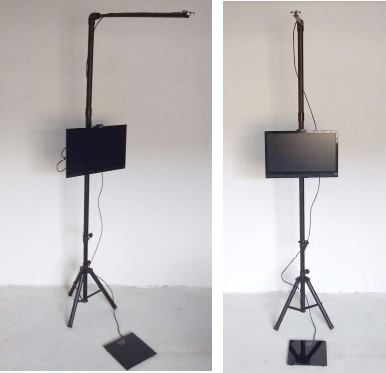
\includegraphics[width=0.90\textwidth]{Figs/Bascula1}
\end{column}
\end{columns}


\end{block} 
\end{frame}


\begin{frame}{\citetitle{MarcoNuno_CongArbEsp_2019_09_01} (3)}

\note[item]{\scriptsize This interface only shows the logo of the device and a welcome message that invitesthe user to starts the interaction through the voice command "HELLO". }
\note[item]{\scriptsize The user only interacts with the system (by voice commands) when physical activity is asked. }
\note[item]{\scriptsize Artificial intelligence models are used to estimate automatically gender and age from camera.}
%\note[item]{\scriptsize The device will ask the user the age, which with the voice, will respond only by saying the user's age (one single number) }
\note[item]{\scriptsize The generated meal plans are only for reference, but the system recommends visiting a nutritionist for further details. }

\begin{block}{Main interface} 
\begin{columns}
\begin{column}{0.3\textwidth}
The shown GUI:
	\begin{itemize}
	\item Represents the actions to be performed by the user. 
    \item Receives the body paramenters of the sensors.
    \item Estimates the BMI.
    \item Proposes a Meal Plan.
	\end{itemize}
\end{column}
\begin{column}{0.7\textwidth}
\begin{center}
     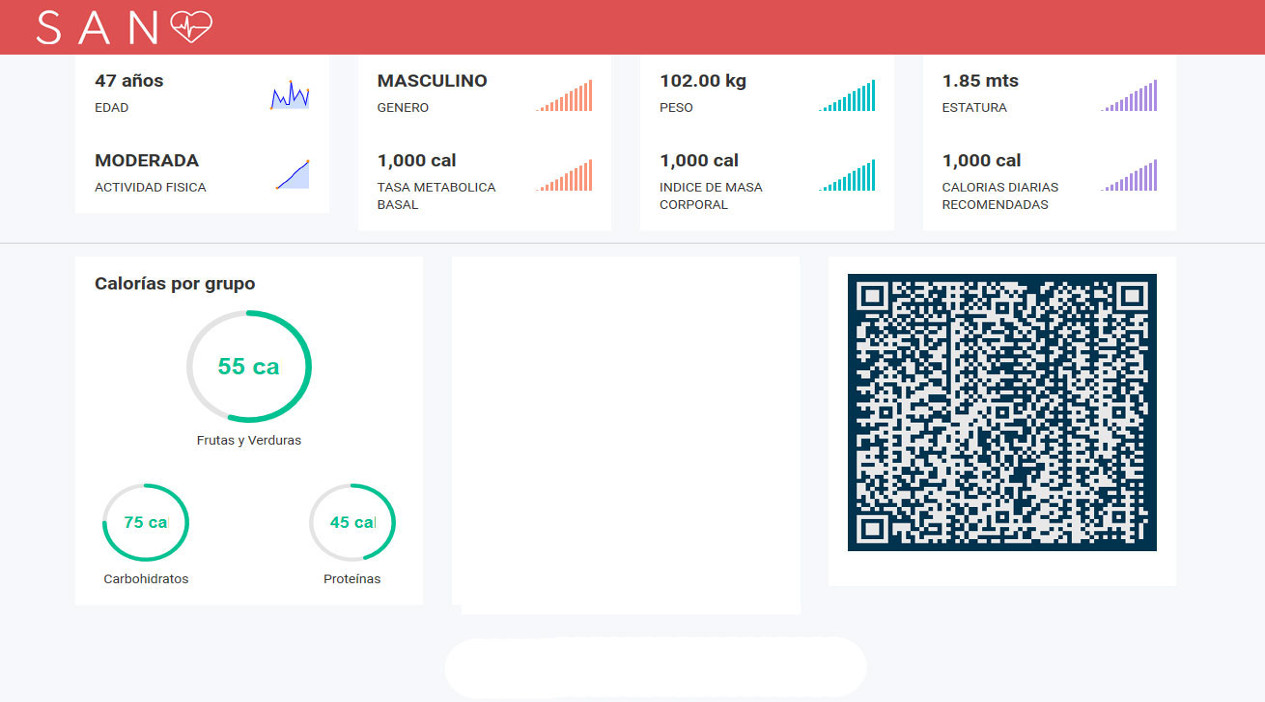
\includegraphics[width=0.99\textwidth]{Figs/Bascula2}
     \end{center}
\end{column}

\end{columns}
\end{block} 
\end{frame}

